\subsection{Założenia projektu:}
\begin{itemize}
	\item \textbf{Lokalizacja}: Grabowno Wielkie (wieś), ulica, na której znajdują się domy o adresach 43-57, 80-90 (włącznie z adresami z literą a) i 121
	\item \textbf{Grupa odbiorców}: Osoby, które to nie mają dużych zapotrzebowań na szybkie łącza internetowe.
	\item \textbf{OLT}: Na wschodzie znajduję się Szkoła Podstawowa, która wydaje się być dobrym miejscem na taką infrastrukturę w tym miasteczku.
	\item \textbf{Swiatłowód}: SM (średnice 8-9 mikrometrów rdzeń, 125 mikrometrów płaszcz)
	\item \textbf{Przepustowość}: 1000Mb/500Mb per end point (budynek). Uwzględnić overbooking na poziomie około 20\%
	\item \textbf{Topologia}: P2MP
	\item \textbf{Architektura}: FTTH
	\item \textbf{System}: GPON
\end{itemize}

\newpage
\subsection{Lokalizacja}

	\begin{center}
		\begin{figure}[h!]
			\makebox[\textwidth]{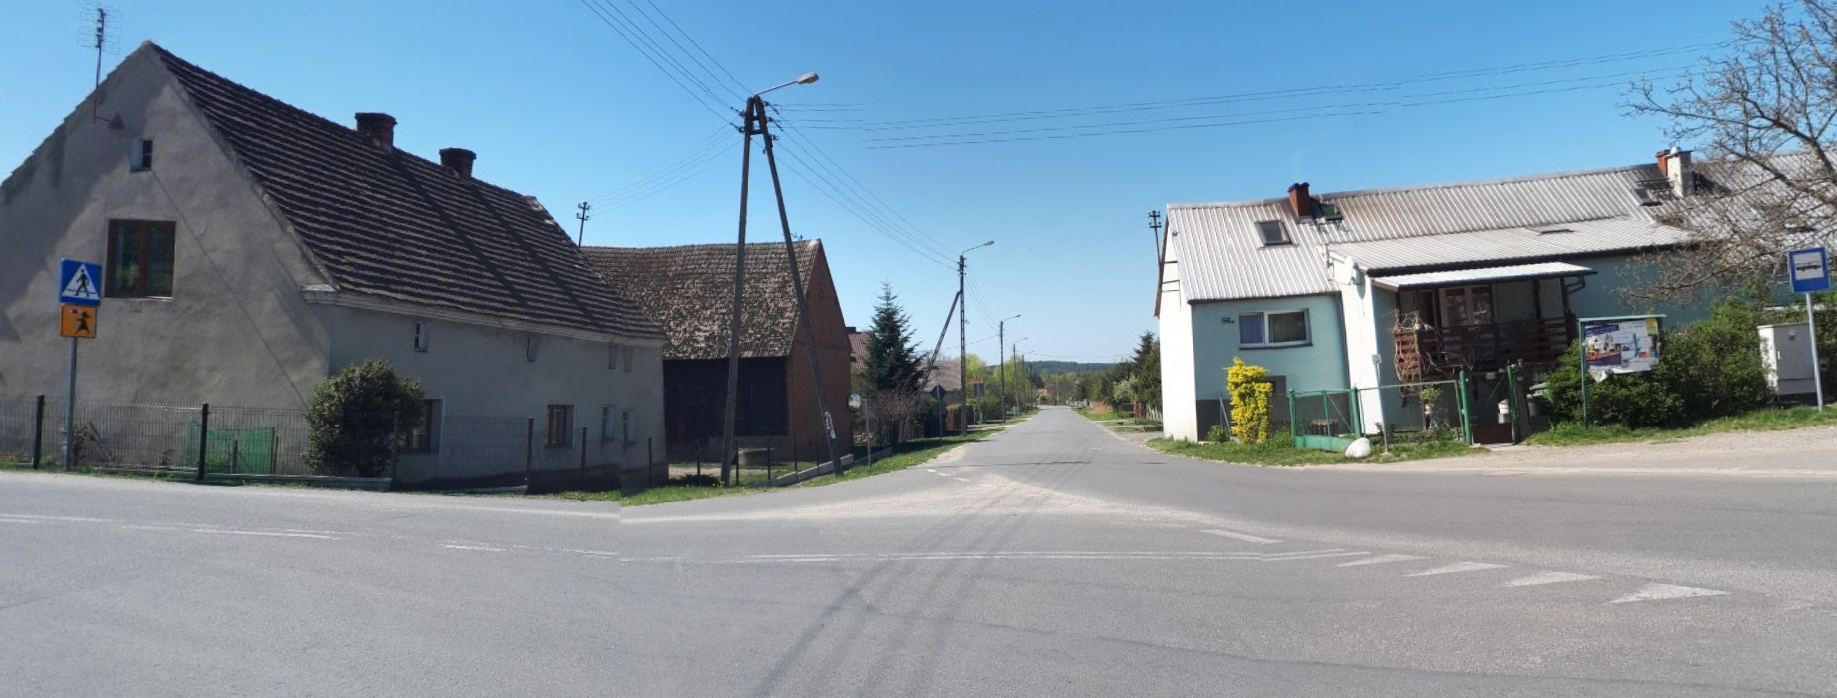
\includegraphics[width=\textwidth]{grabowno_intro.png}}
			\caption{Grabowno Wielkie}
			\label{fig:grabowno_intro}
			\begin{center}\cite{grabowno_intro}\end{center}
		\end{figure}
	
		\begin{figure}[h!]
			\makebox[\textwidth]{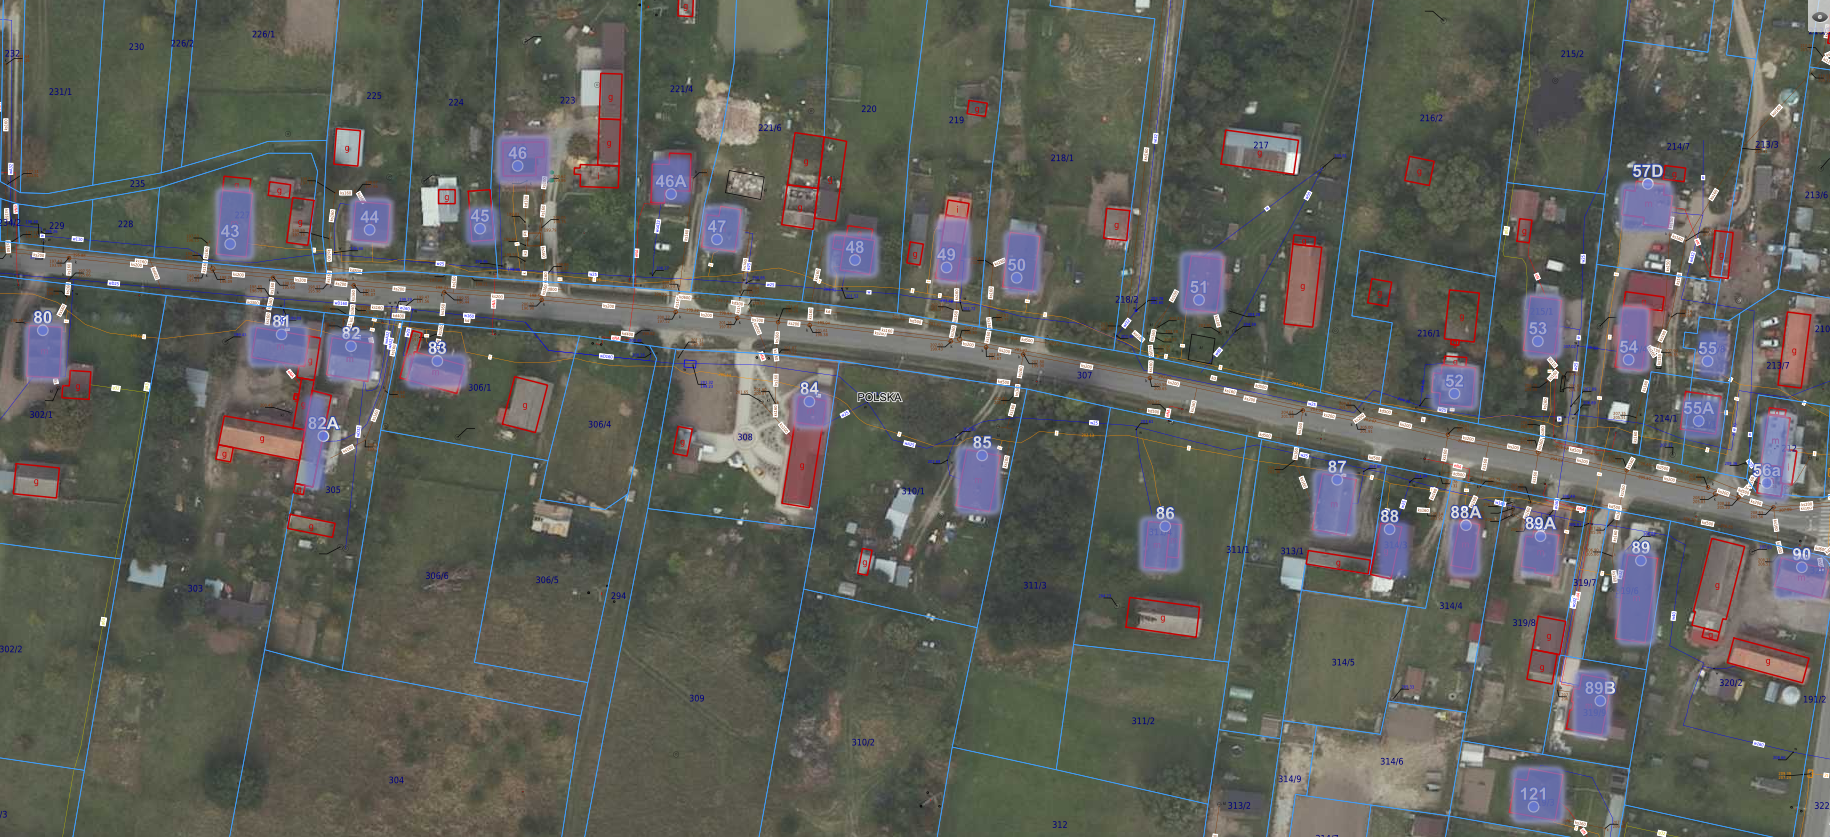
\includegraphics[width=\textwidth]{plan_intro.png}}
			\caption{Plan wsi}
			\label{fig:plan_intro}
			\begin{center}\cite{plan_intro}\end{center}
		\end{figure}
	
	\end{center}

	Numery działek mające zostać objęte siecią:
	\begin{itemize}
		\item od północnej strony ulicy numery od 43 do 57
		\item od południowej strony numery od 80 do 90 oraz 121
	\end{itemize}
